\section{Countermeasures}
A possible countermeasure against \bc detection is to tunnel \bc traffic over 
an anonymity system like Tor. We tunnel \bc traffic over Tor to disguise its patterns. We evaluate the invisibility that Tor provides by designing a new classifier (SizeTor) which is tailored for Tor. Also, we use our strongest classifiers (NN-based and combined) to evaluate if Tor succeeds in hiding \bc traffic.

%We design a new classifier to detect \bc in a case that it is tunneled over Tor. Also, we use our NN-based model introduced in Section~\ref{class:nn} to detect \bc when it is tunneled over Tor.
\subsection{Bitcoin Over Tor}\label{sec:tor}
Tor sends traffic in \textit{cells}. If the packets sizes is below the cell size, it will add padding to the packets to reach the fixed cell sizes. This modifies the traffic patterns of \bc traffic, e.g., its packet sizes, therefore it may increase resistance to traffic classification. 
In the following we evaluate our classifiers against Tor and three state-of-the-art Tor 
pluggable transports~\cite{pluggable-transport} namely \textit{obfs4}, \textit{FTE}, and \textit{Meek} explained in the following. 

\paragraphb{Pluggable Transports:} We evaluated against the following major transports:
\begin{compactitem}
\item	\textbf{Obfs4:}
obfs4 is a widely used Tor pluggable transport, which is based on \textit{ScrambleSuit}~\cite{scramblesuit}. It differs with ScrambleSuit in public key obfuscation and its protocol for one-way authentication, which makes it faster. 
\item \textbf{FTE} 
The FTE transport re-encrypts Tor packets in order to match the regular expressions of a benign protocol like HTTP. 
\item\textbf{meek}
Meek uses \textit{domain fronting}~\cite{meek-PETS} to tunnel traffic through public CDN or cloud platforms. 
\end{compactitem}
\begin{figure}
\centering
\begin{subfigure}{0.48\linewidth}
\centering
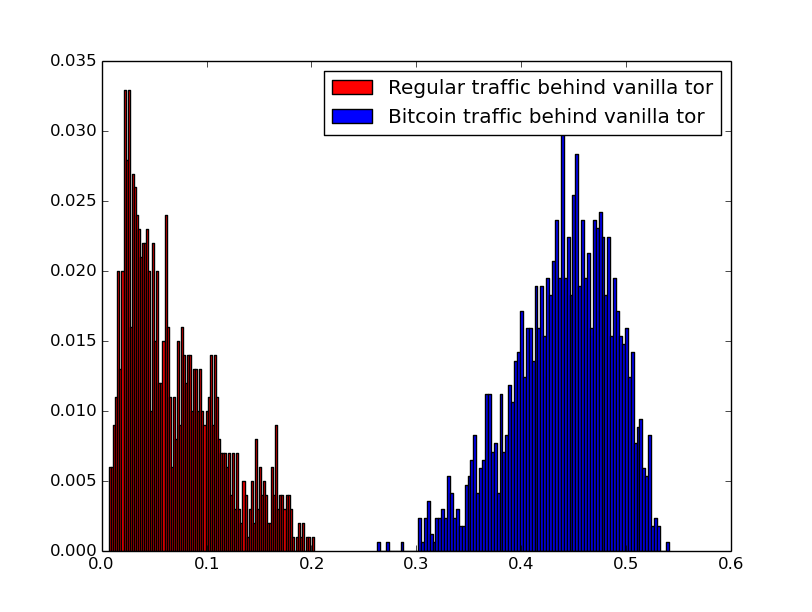
\includegraphics[width=\linewidth]{image/ratio_609_upstream_compact_vanilla_tor.png}
\caption{upstream}
\label{fig:ratio_609_upstream_compact_vanilla_tor}
\end{subfigure}
\begin{subfigure}{0.48\linewidth}
\centering
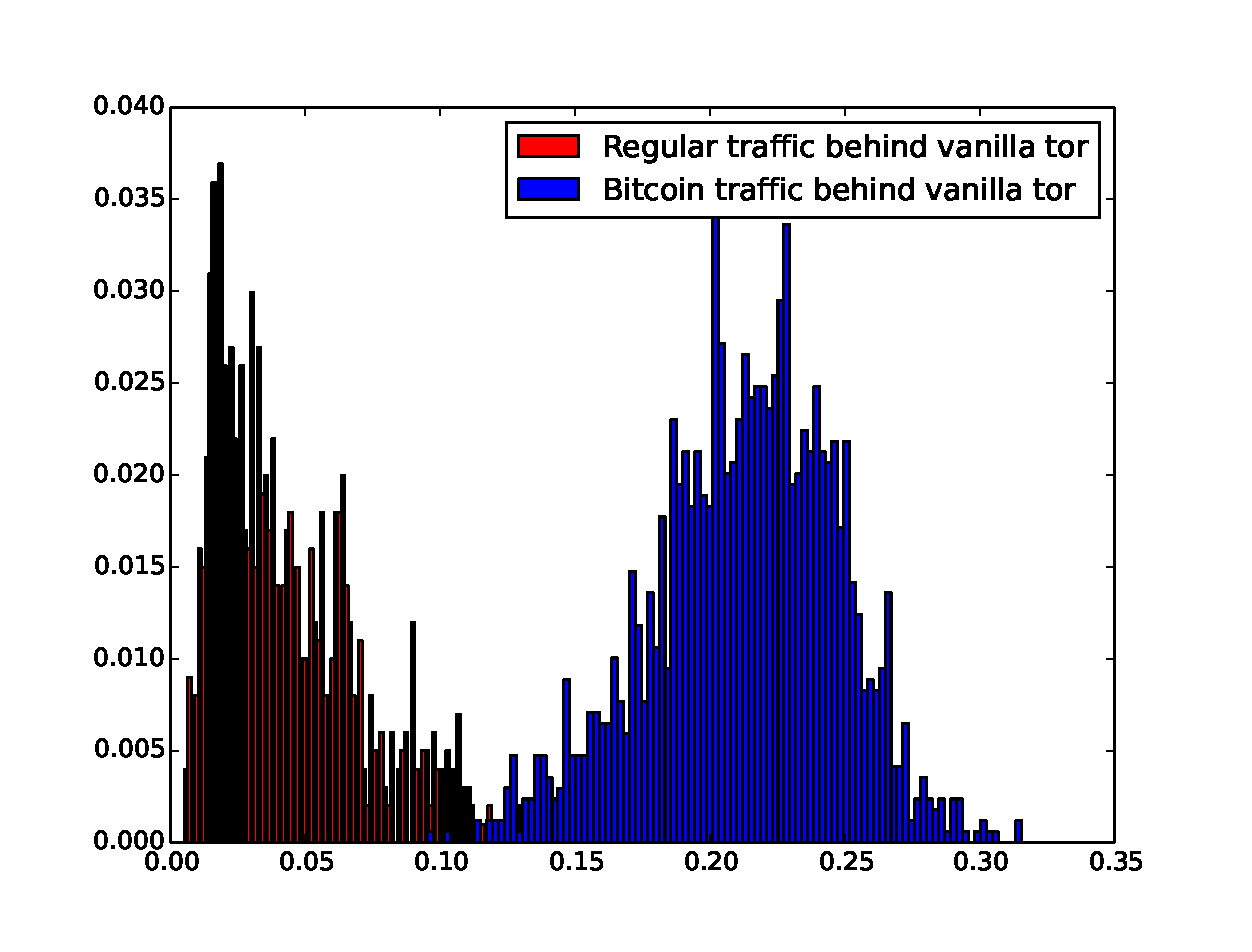
\includegraphics[width=\linewidth]{image/ratio_609_downstream_compact_vanilla_tor.eps}
\caption{downstream}
\label{fig:ratio_609_downstream_compact_vanilla_tor}
\end{subfigure}
\caption{Histogram of one cell packet ratio for HTTP traffic and \bc traffic}
\end{figure}
\bc traffic has a larger ratio of one-cell packets compared to Tor. This is due to a large number of small \bc messages (e.g., \code{inv}) that are each put into a single-cell packets. Figures \ref{fig:ratio_609_upstream_compact_vanilla_tor} and \ref{fig:ratio_609_downstream_compact_vanilla_tor} show the histogram of one cell size packets ratio in the upstream and downstream directions.

%As it is shown in Appendix~\ref{sec:charachterzing_bc}, the distribution of packet sizes differs in \bc and other types of traffic. While Tor modifies the sizes of \bc traffic, it does not remove all traffic patterns that reveal \bc. 

\iffalse, we show that this does not remove all traffic patterns that reveal \bc. We compare the distribution of packet sizes in HTTP traffic and \bc traffic behind Tor. 
Figures~\ref{fig:tor_reg_traffic_pkt_size_upstream} to \ref{fig:tor_compact_block_pkt_size_downstream} in Appendix~\ref{sec:bcshape} compare the distribution of packet sizes of HTTP and \bc when tunneled over Tor in different modes, showing an identifiable pattern.\fi
 
\subsection{Evaluating \bc over Tor}
\paragraphb{\code{SizeTor} classifier}
We implement ~\code{SizeTor} classifier on noisy \bc on compact mode for Tor and its three pluggable transports. As it is displayed in Figure~\ref{fig:tor_sizeTor}, we could detect \bc traffic with high accuracy for the complex user model when the background noise is one open tab. As Figure~\ref{fig:tor_sizeTor} indicates, having a traffic size of $10$ minutes is
enough to detect \bc traffic with around $90\%$ true positive and $0\%$ of false positive. Moreover, the Figure states that the result of classifier quickly diminishes when we increase the background noise from one to $2$ or $3$ open tabs.
Note that this figure shows the average result of this classifier on Tor and three pluggable transports.

\paragraphb{Neural Network-based classifier}
Table~\ref{tab:nn_tor} presents the result of NN-based classifier for the complex web user over Tor for $10,000$ numbers of test data. As the table suggests, performance of our classifier improves when we increase the size of training data. More specifically, our false positives enhances from $11\%$ to $4\%$ when we increase the training data from $1000$ to $40,000$. Moreover, when using $40,000$ training data, we reach $99\%$ and $4\%$ true and false positive, respectively ($97\%$ accuracy). Note that the reason we get better results from this classifier on Tor dataset is that this dataset only contains the complex web user since we did not have CAIDA application over Tor to use for our evaluation.
\begin{comment}
\begin{table}[h!]
  \begin{center}
     \caption{Result of Neural Network classifier for Tor dataset}
    \label{tab:nn_tor}
    \begin{tabular}{c|c|c|c}
    \kern 0.5pc \shortstack{ Training \\Size}& \shortstack{False Positive\\ ($\%$)} &\shortstack{True Positive\\ ($\%$)}&\shortstack{Accuracy \\($\%$)} \kern 0.5pc\\
      \hline
	$1000$&$11$ &$98 $  & $93$\\
	$5000$&$6$& $98$  & $96$\\
	$10,000$&$3$& $98$  &$ 97$\\
	$40,000$&$4$& $99$   & $97$\\
    \end{tabular}
  \end{center}
\end{table}
\end{comment}
\begin{table}
\center \caption{Result of neural network classifier on Tor dataset.}\label{tab:nn_tor}
\begin{tabular}{|c|c|c|c|}
\hline
 Training size& False positive ($\%$) &True positive ($\%$)&Accuracy ($\%$)\\
      \hline
	$1000$&$11$ &$98 $  & $93$\\
	$5000$&$6$& $98$  & $96$\\
	$10,000$&$3$& $98$  &$ 97$\\
	$40,000$&$4$& $99$   & $97$\\
\hline
\end{tabular}
\end{table}


\begin{figure}
\centering
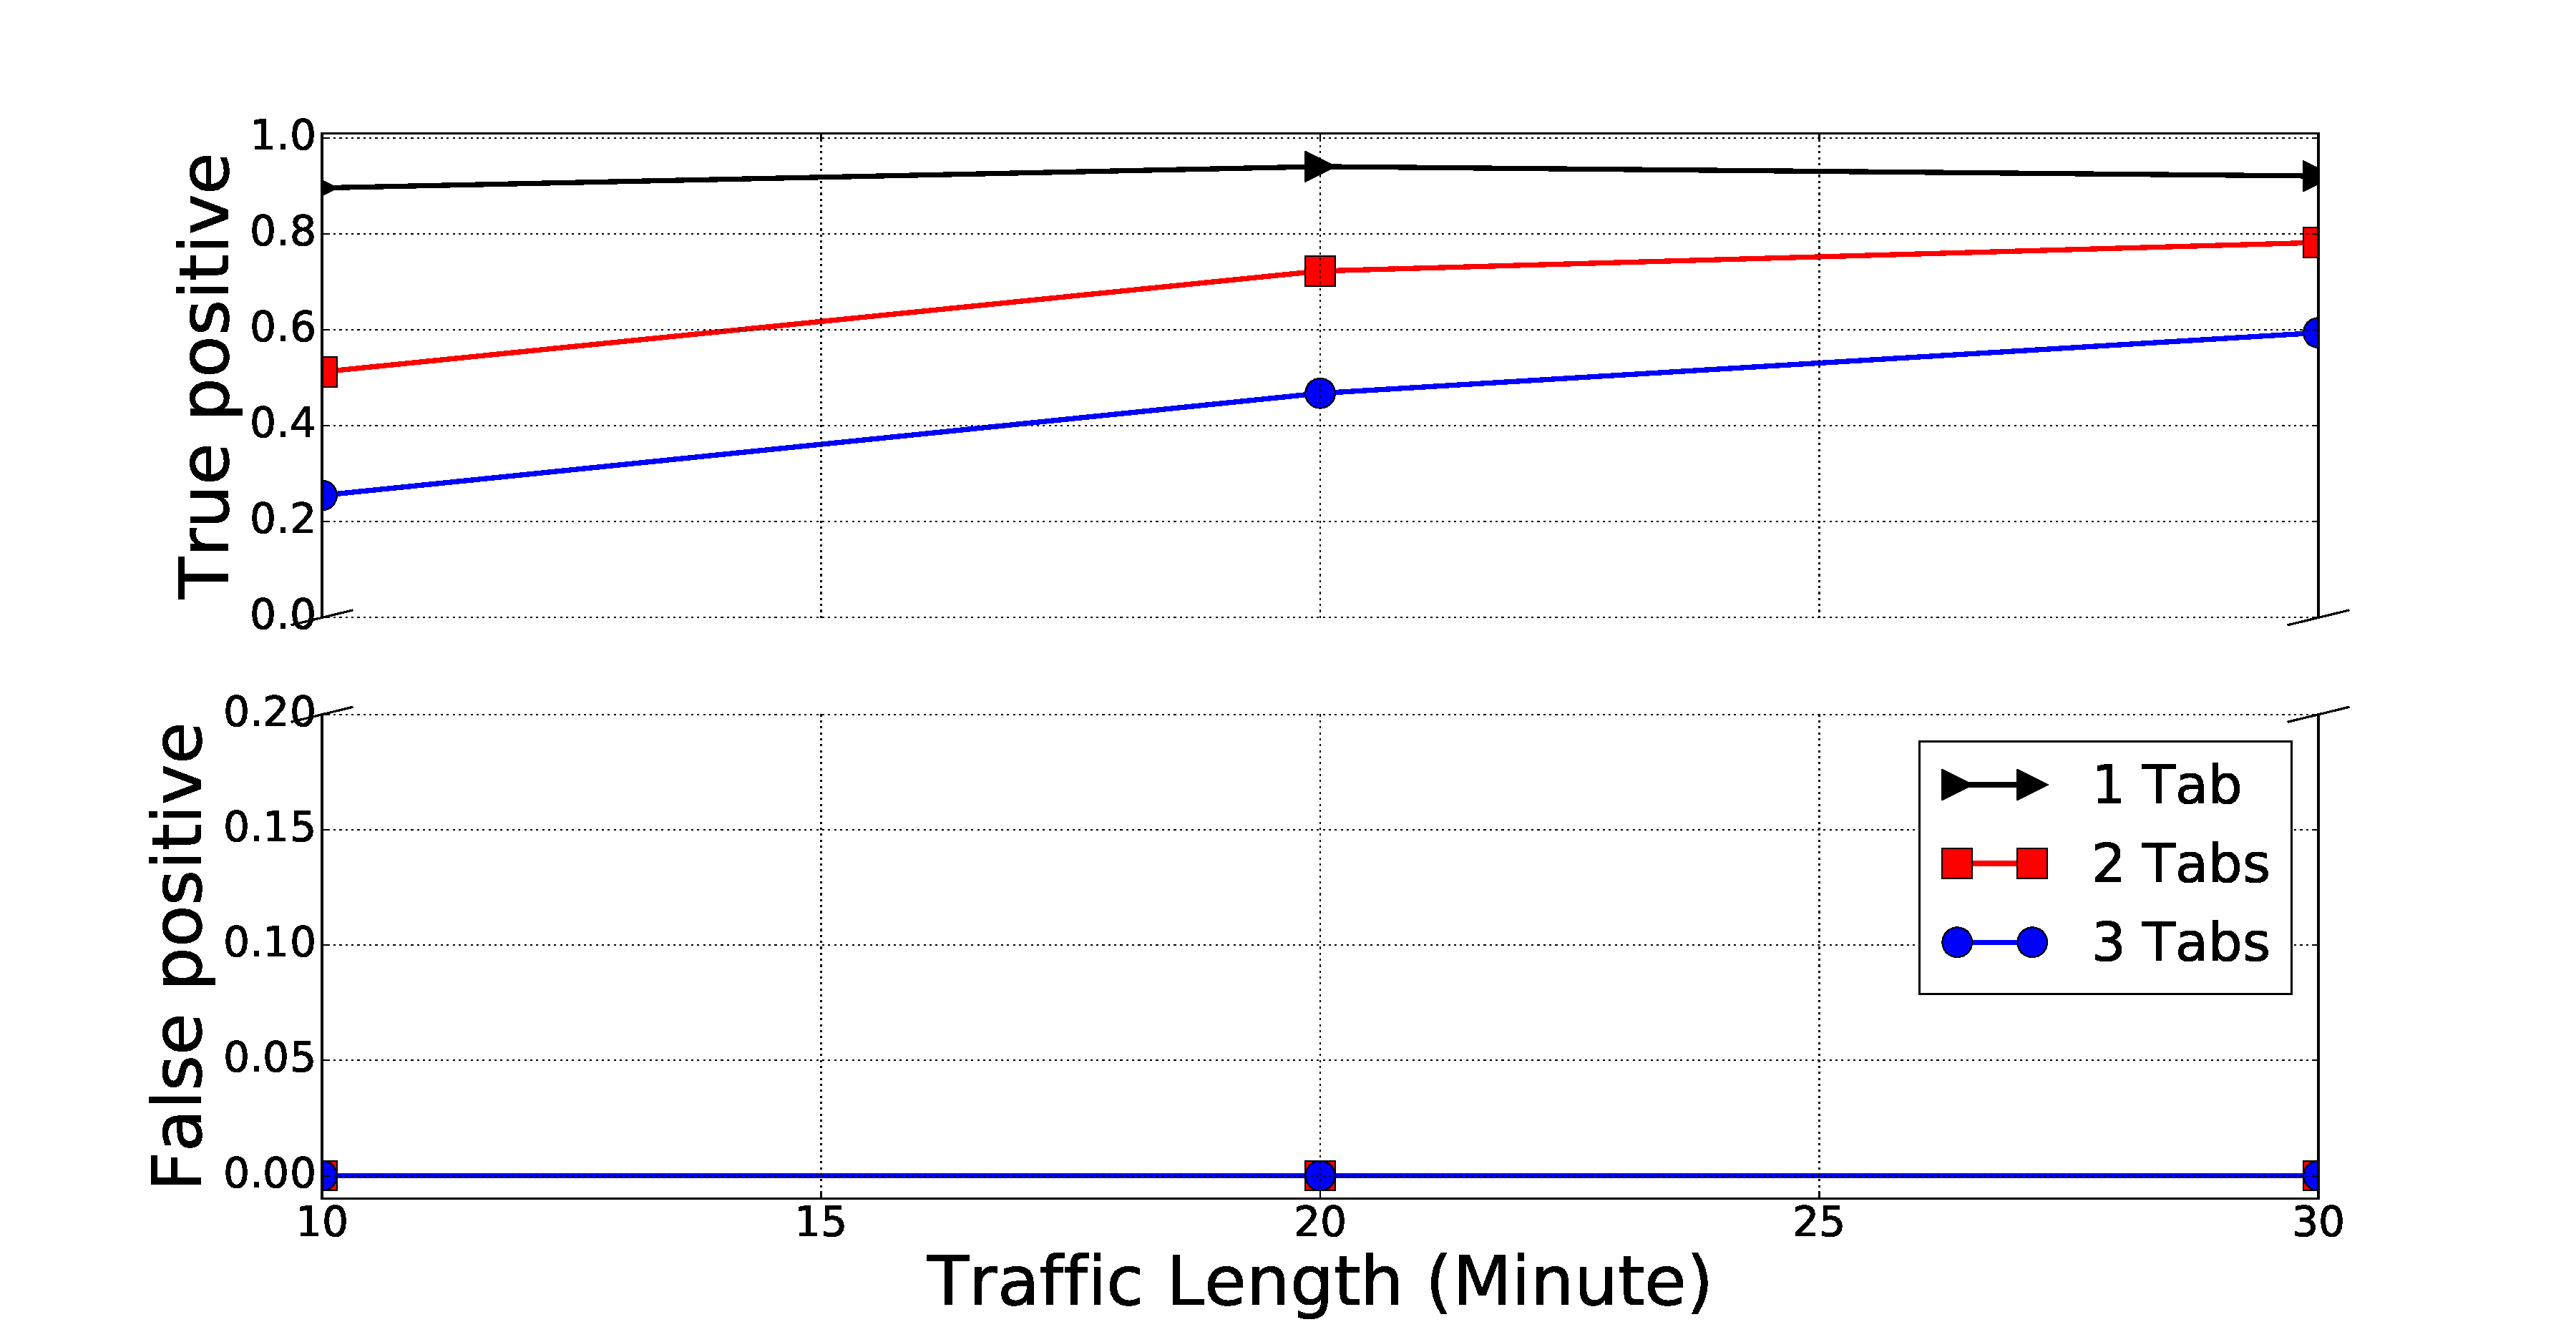
\includegraphics[scale=0.15]{image/jan25/sizeTor-multiTab.pdf}%roc is also available
\caption{Detecting Bitcoin compact mode traffic behind Tor (Tor and its three pluggable transports: meek, obfs, fte) using SizeTor}
\label{fig:tor_sizeTor}
\end{figure}


\iffalse
\subsection{Bitcoin over VPN}
Another countermeasure that we evaluate is passing our traffic through VPN. Since VPN encrypts the traffic and 
\subsubsection{Evaluating Bitcoin over VPN}


\begin{figure*}[!t]
\begin{subfigure}{.48\linewidth}
\centering
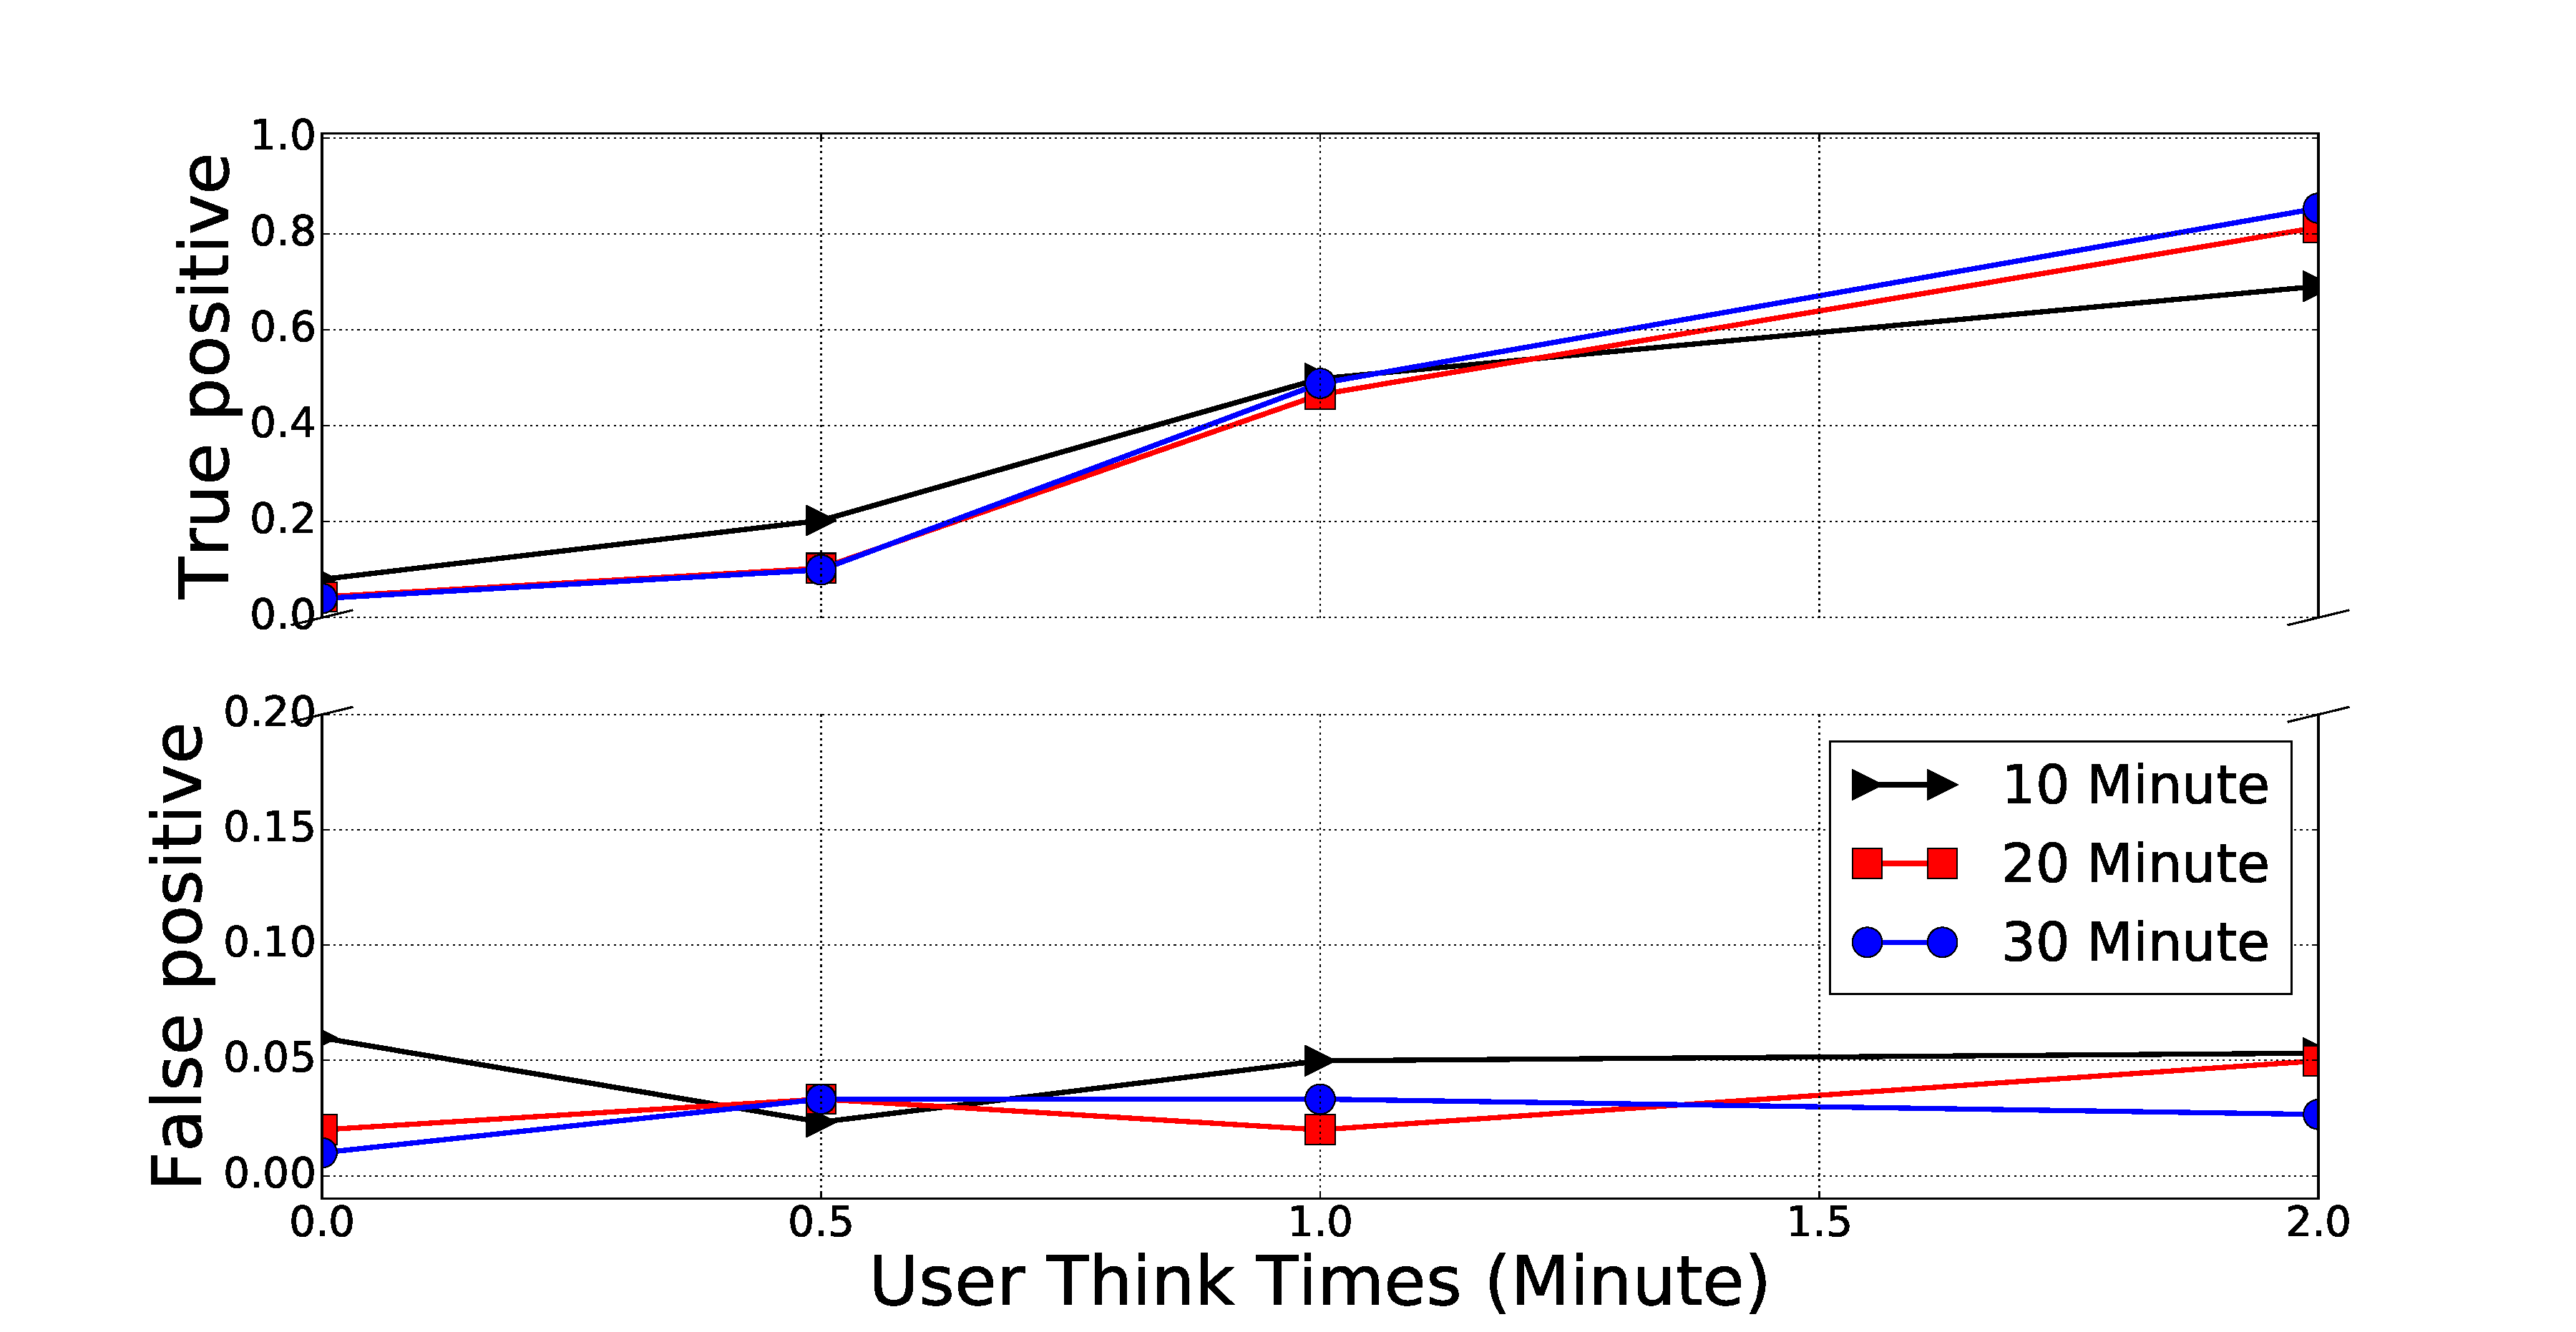
\includegraphics[width=\linewidth]{image/jan25/vpn_d2u.pdf}
\caption{Result of \code{D2U} classifier according to traffic length and think time}
\label{fig:tp}
\end{subfigure}
\centering
\begin{subfigure}{.48\linewidth}
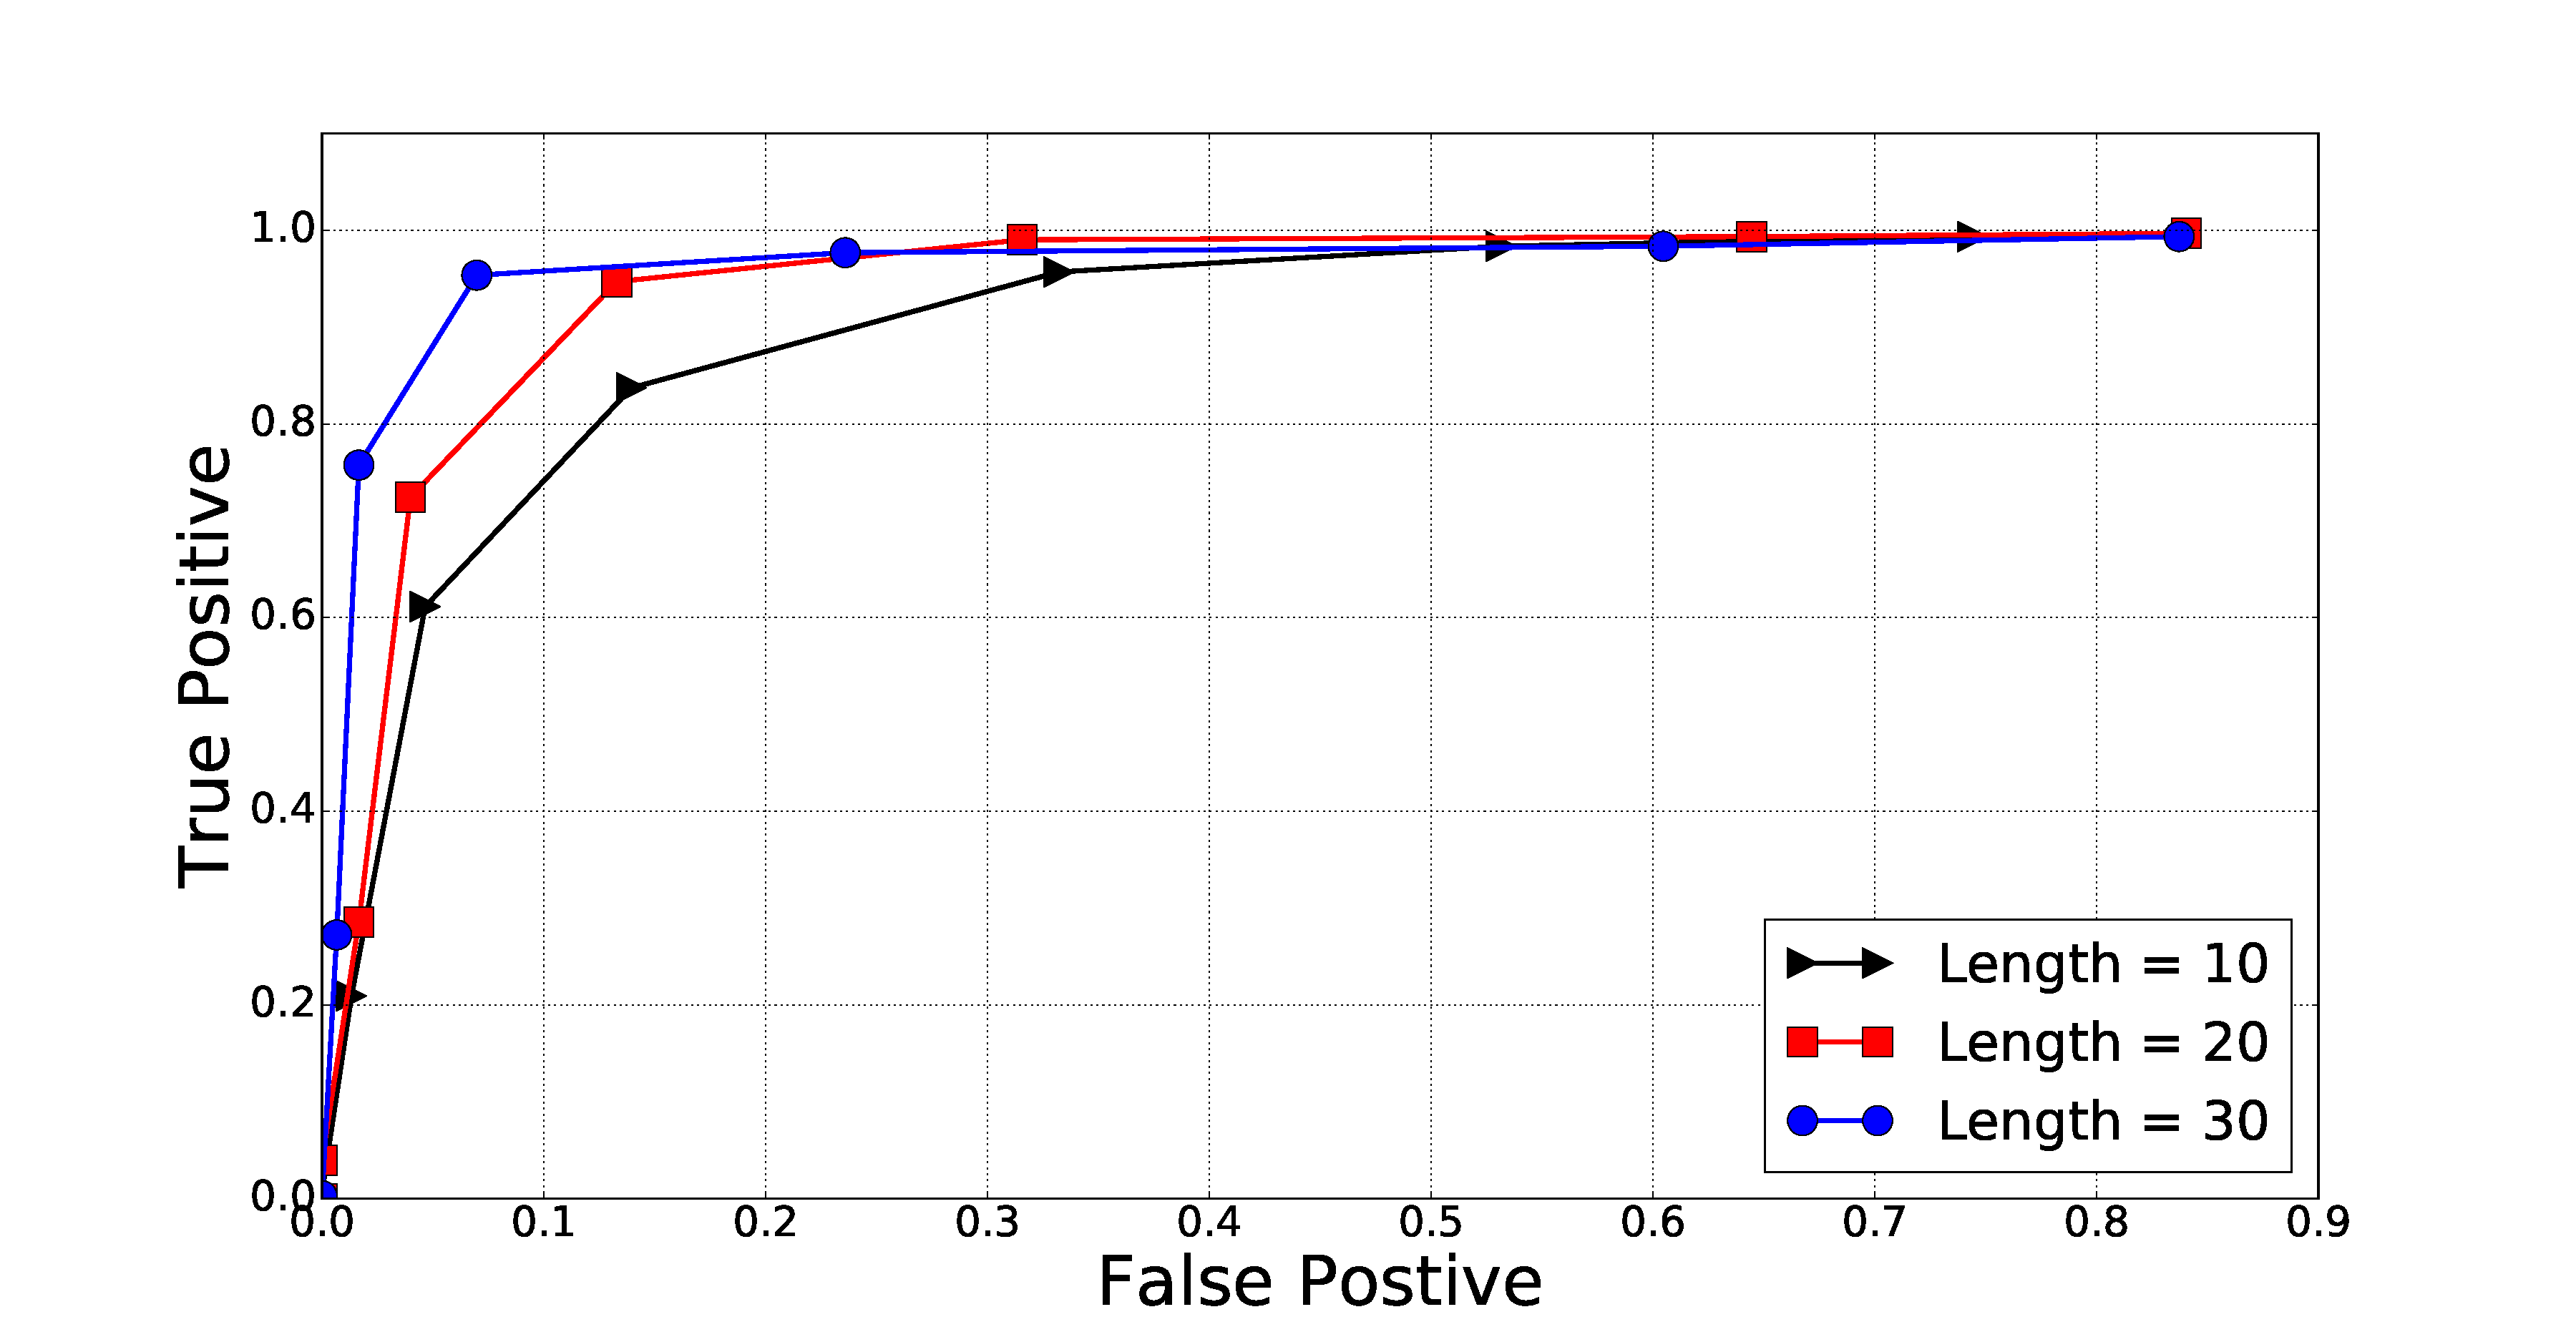
\includegraphics[width=\linewidth]{image/jan25/roc_vpn_d2u.pdf}
\caption{ROC curve for Think Time $=2$ minutes}
\label{fig:fp}
\end{subfigure}
\caption{Result of \code{D2U} classifier on \bc Traffic Tunneled over VPN}
\label{fig:vpn}
\end{figure*}
\fi





\paragraphb{Combined classifier over Tor}
We apply the combined classifier on our Tor dataset, which consists of \bc traffic with up to $5$ number of open tabs on the background. Our experiments show that having $40,000$ of training data is enough to achieve more than $99.72\%$ accuracy with $0.04\%$ false positive and $99.5\%$ true positive. Our combined classifier outperforms the previous classifiers (SizeTor and NN-based) on the Tor dataset as well. This is because we are using a more complex model and a more significant number of features.


\begin{comment}
\begin{table}
\center \caption{Result of combined classifier over Tor.}\label{tab:comb_t}
\begin{tabular}{|c|c|c|c|}
\hline
 Training size& False positive ($\%$) &True positive ($\%$)&Accuracy ($\%$)\\
      \hline
    $1000$    &$0.22$   & $71.36$   & $83.95$\\% for 50 epochs

	$5000$    &$0.79$   & $99.91$   & $99.6$\\% for 50 epochs
	$10,000$  &$0.0$   & $99.91$   & $99.95$\\% for 50 epochs
	$20,000$  &$0.0$  & $99.76$   & $99.84$\\% for 50 epochs
\hline
\end{tabular}
\end{table}

\end{comment}






%Figure~\ref{fig:d2u-Tor} shows the performance of our \code{D2U} classifier for the three transports, showing that it can reliably distinguish \bc traffic when there is HTTP browsing noise on the background. As it is shown from the figure, we are able to distinguish the \bc traffic with good accuracy in presence of background noise. 

\begin{comment}

Furthermore, We implement the D2U and SizeHist classifier on \bc traffic tunneled over Tor (Tor and three pluggable transports).
Figure~\ref{fig:tor_d2u} shows the result of the \code{D2U} classifier on \bc traffic (in compact block mode) tunneled over Tor.
Figure~\ref{fig:plug_tor_dow_up_ratio} shows the histogram of downstream-to-upstream traffic for \bc and HTTP using the three pluggable transports (no background noise). As can be seen, in the absence of the background noise there is a wide gap between the histograms of \bc and HTTP, allowing us to use the \code{D2U} classifier. Thus, we implemented \code{D2U} classifier for \bc traffic tunneled over three Tor pluggable transports. Figure~\ref{fig:tor_d2u} shows the average of result of this classifier for Tor and its three pluggable transports. The figure indicates that we can detect \bc traffic in presence of normal background noise with more than $0.80$ percent accuracy when we have $10$ minutes of \bc traffic and we can reach perfect accuracy when we increase the traffic length to $30$ minutes.


\begin{figure*}
\begin{subfigure}{0.32\linewidth}
\centering
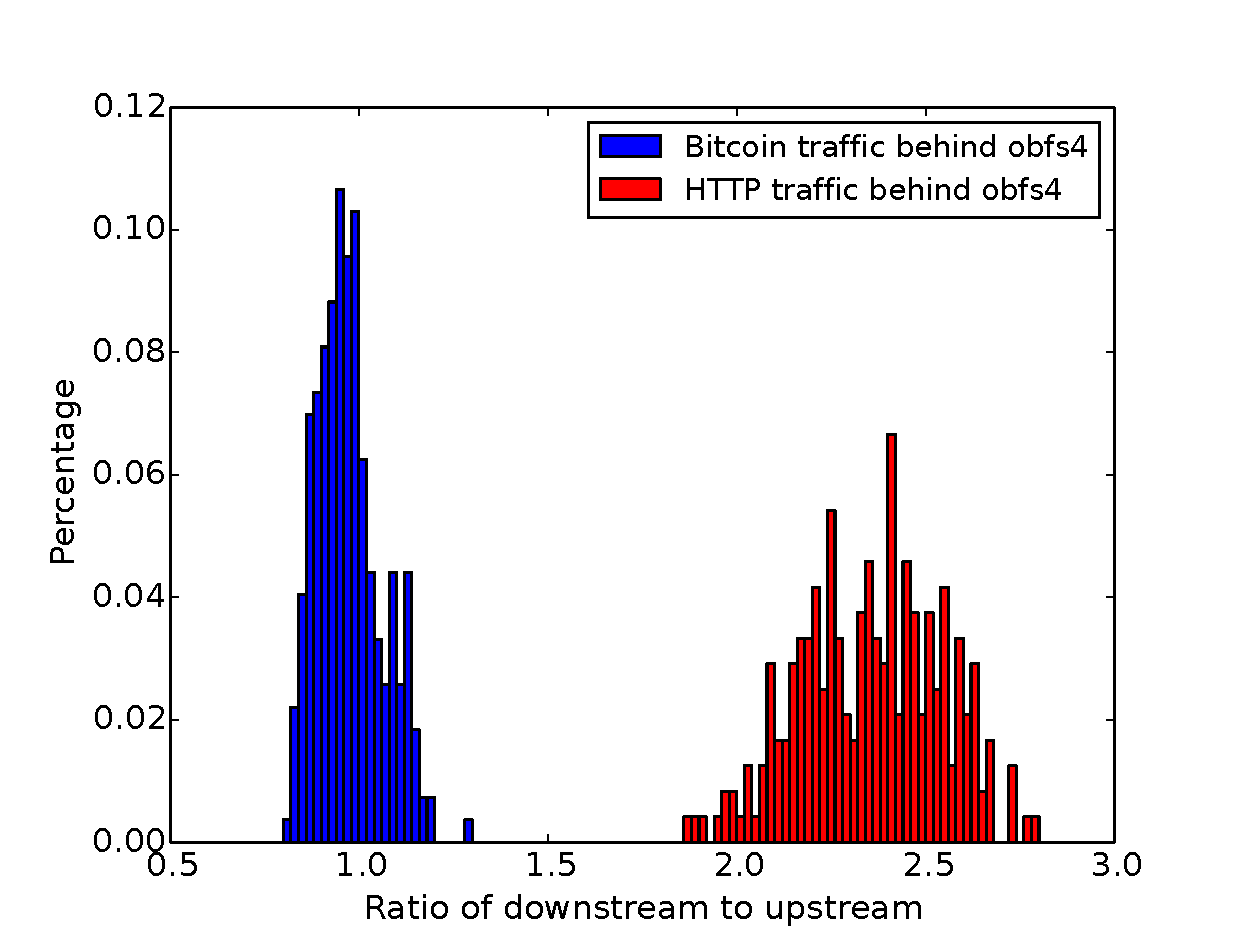
\includegraphics[width=\linewidth]{image/obfs4_corr_value_btc_http.eps}
\caption{Obfs4}
\label{fig:obfs4_corr_value_btc_http}
\end{subfigure}
\begin{subfigure}{0.32\linewidth}
\centering
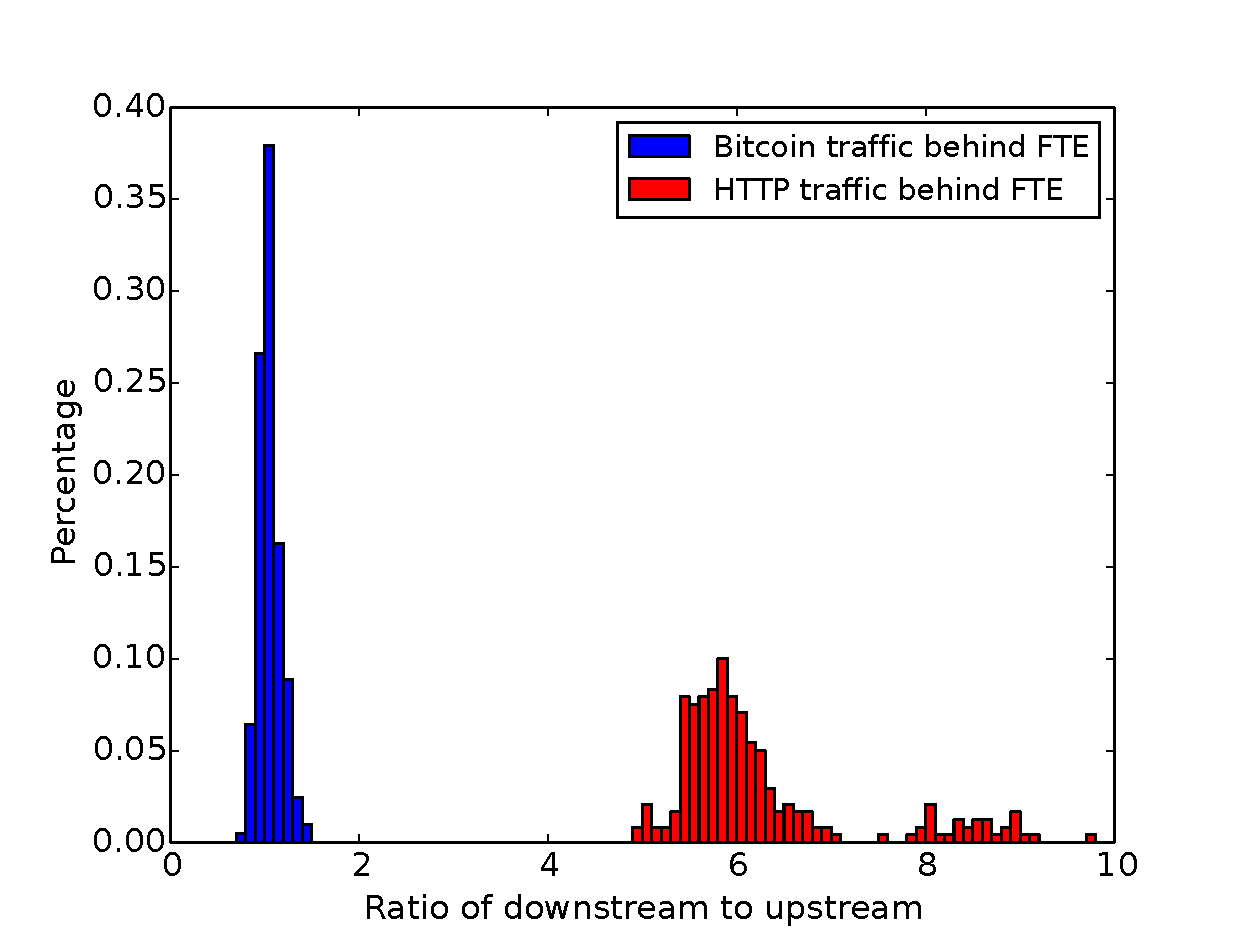
\includegraphics[width=\linewidth]{image/fte_corr_value_btc_http.eps}
\caption{FTE}
\label{fig:fte_corr_value_btc_http}
\end{subfigure}
\begin{subfigure}{0.32\linewidth}
\centering
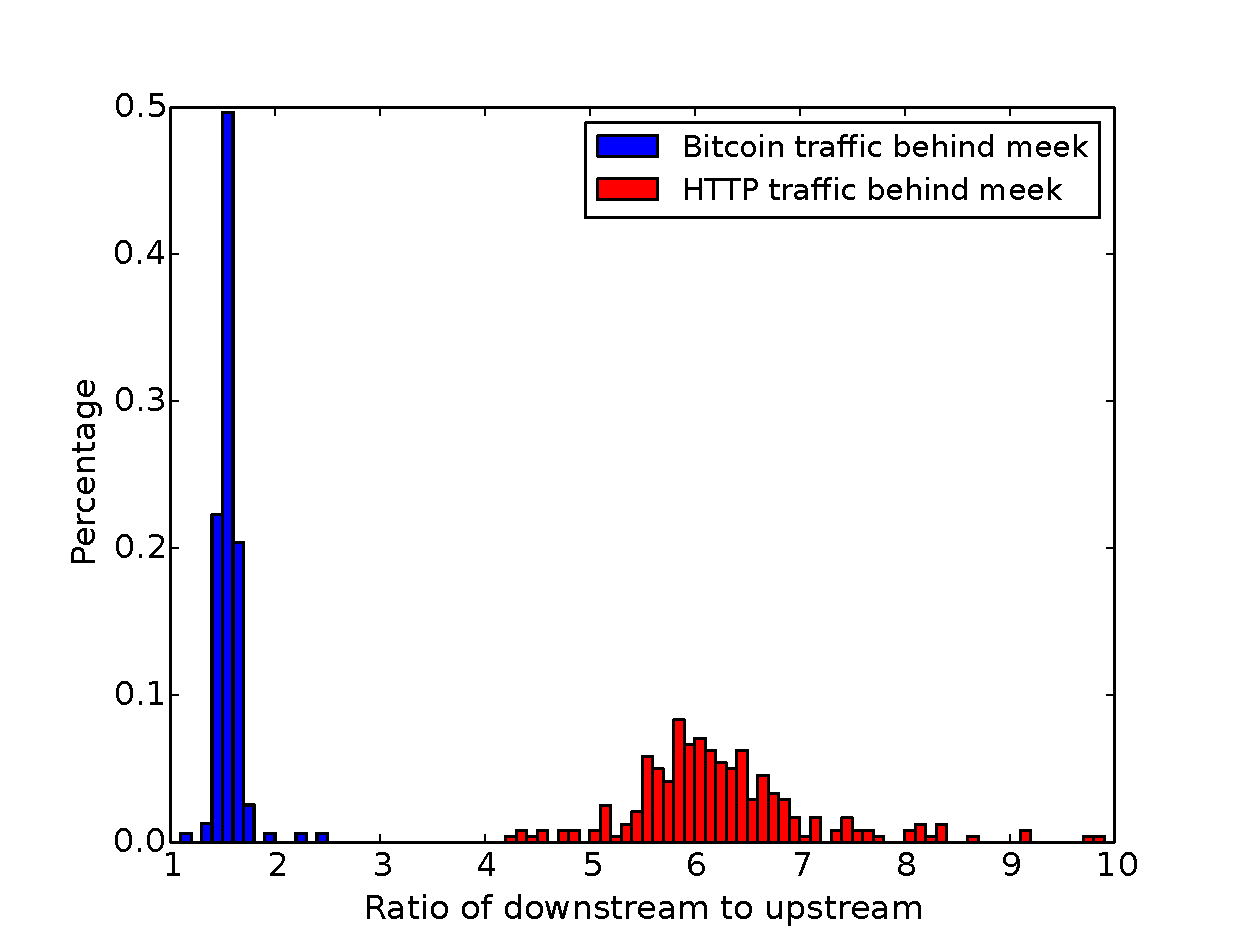
\includegraphics[width=\linewidth]{image/meek_corr_value_btc_http.eps}
\caption{Meek}
\label{fig:meek_corr_value_btc_http}
\end{subfigure}
\caption{Histogram of downstream to upstream ratio for 30 minutes of traffic}
\label{fig:plug_tor_dow_up_ratio}
\end{figure*} 
\end{comment}

\begin{comment}
\begin{figure*}
\begin{subfigure}{0.32\linewidth}
\centering
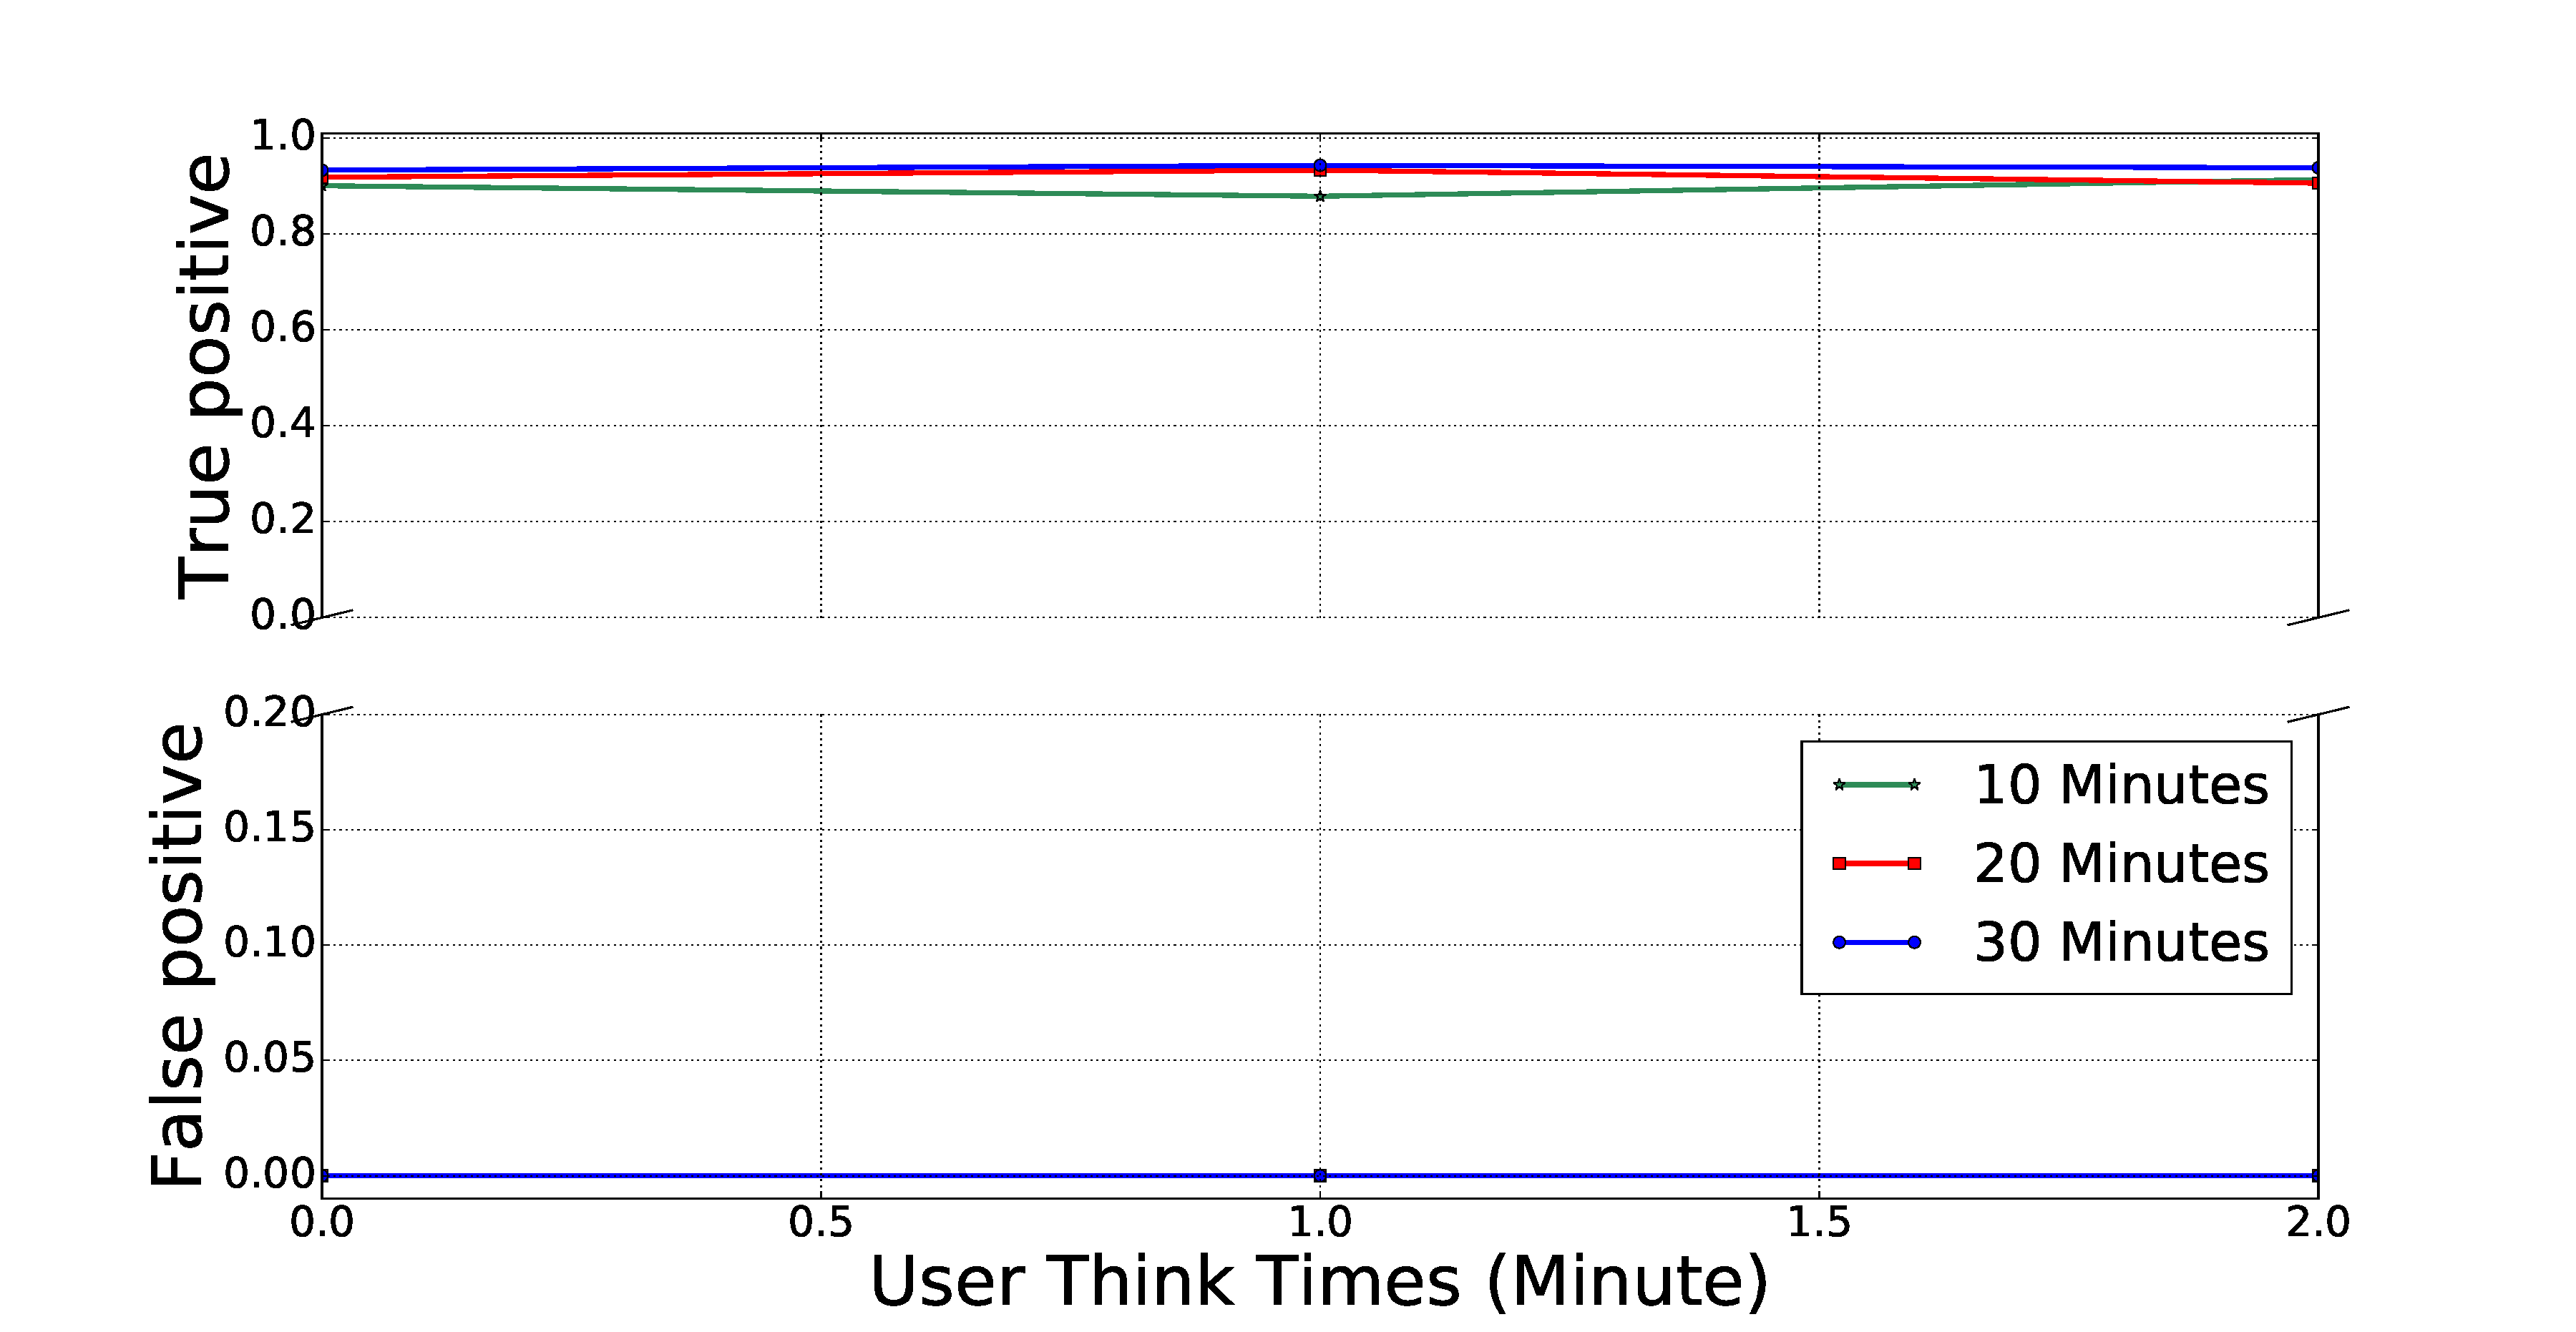
\includegraphics[width=\linewidth]{image/jan25/tor_all_sizetor.pdf}
\caption{SizeTor}
\label{fig:tor_sizeTor}
\end{subfigure}
\begin{subfigure}{0.32\linewidth}
\centering
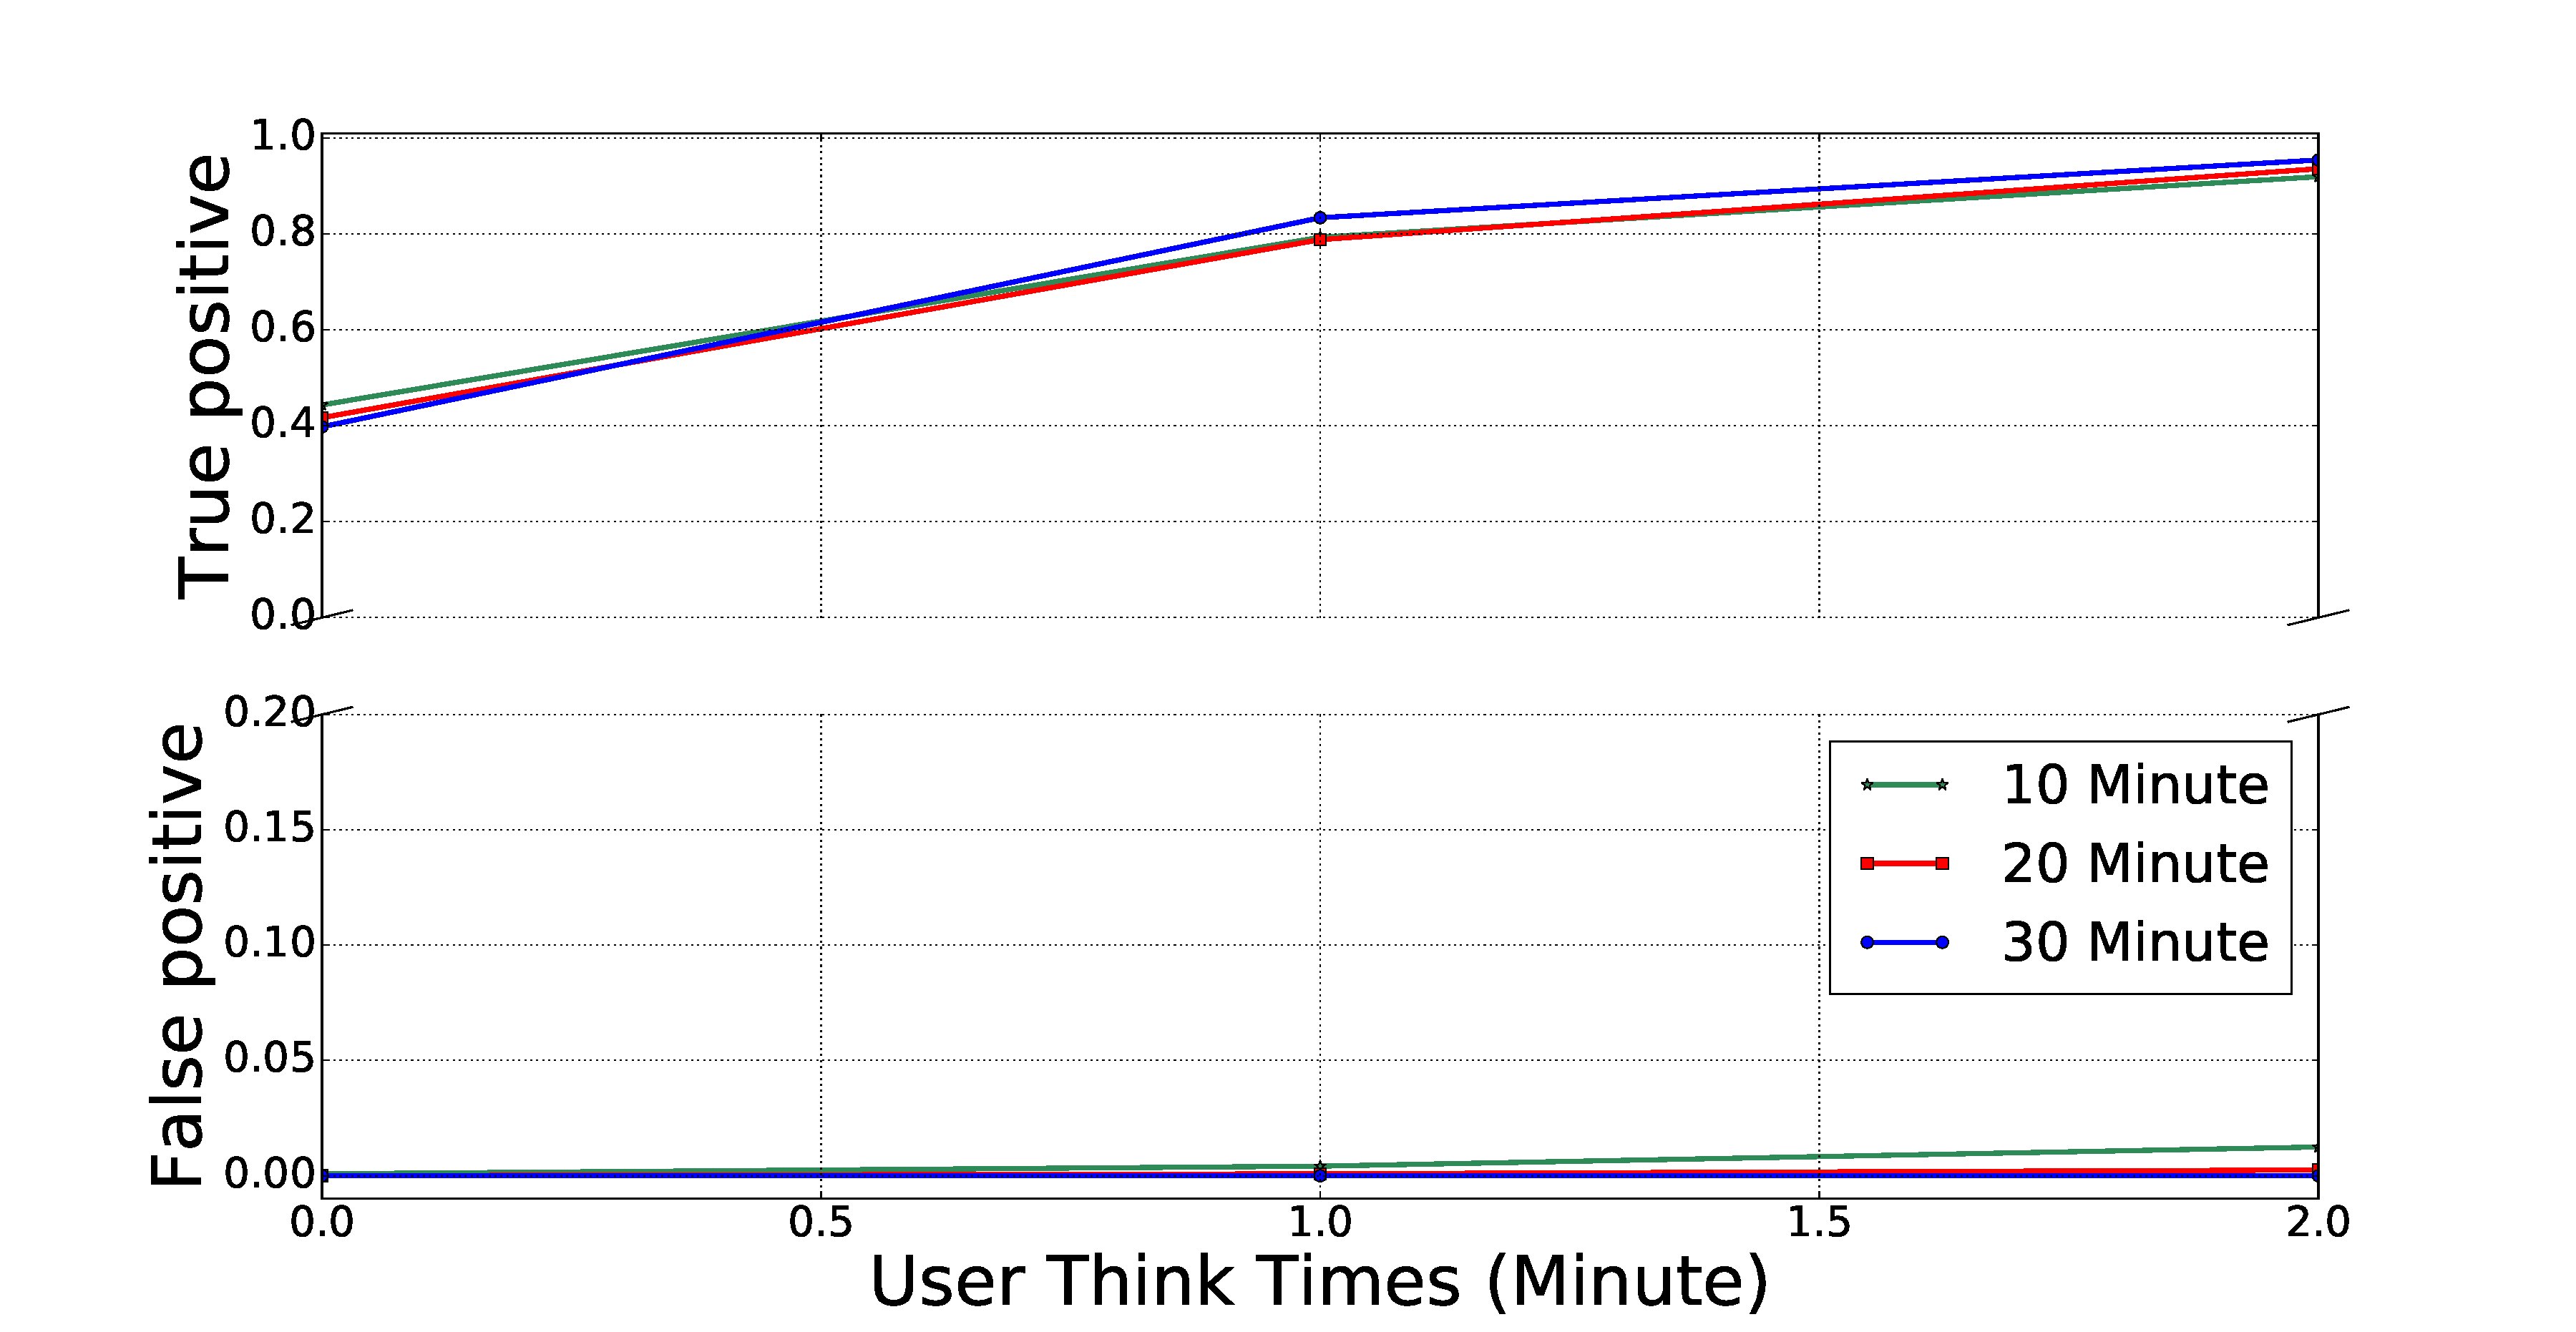
\includegraphics[width=\linewidth]{image/jan25/tor_all_d2u.pdf}
\caption{D2U}
\label{fig:tor_d2u}
\end{subfigure}
\begin{subfigure}{0.32\linewidth}
\centering
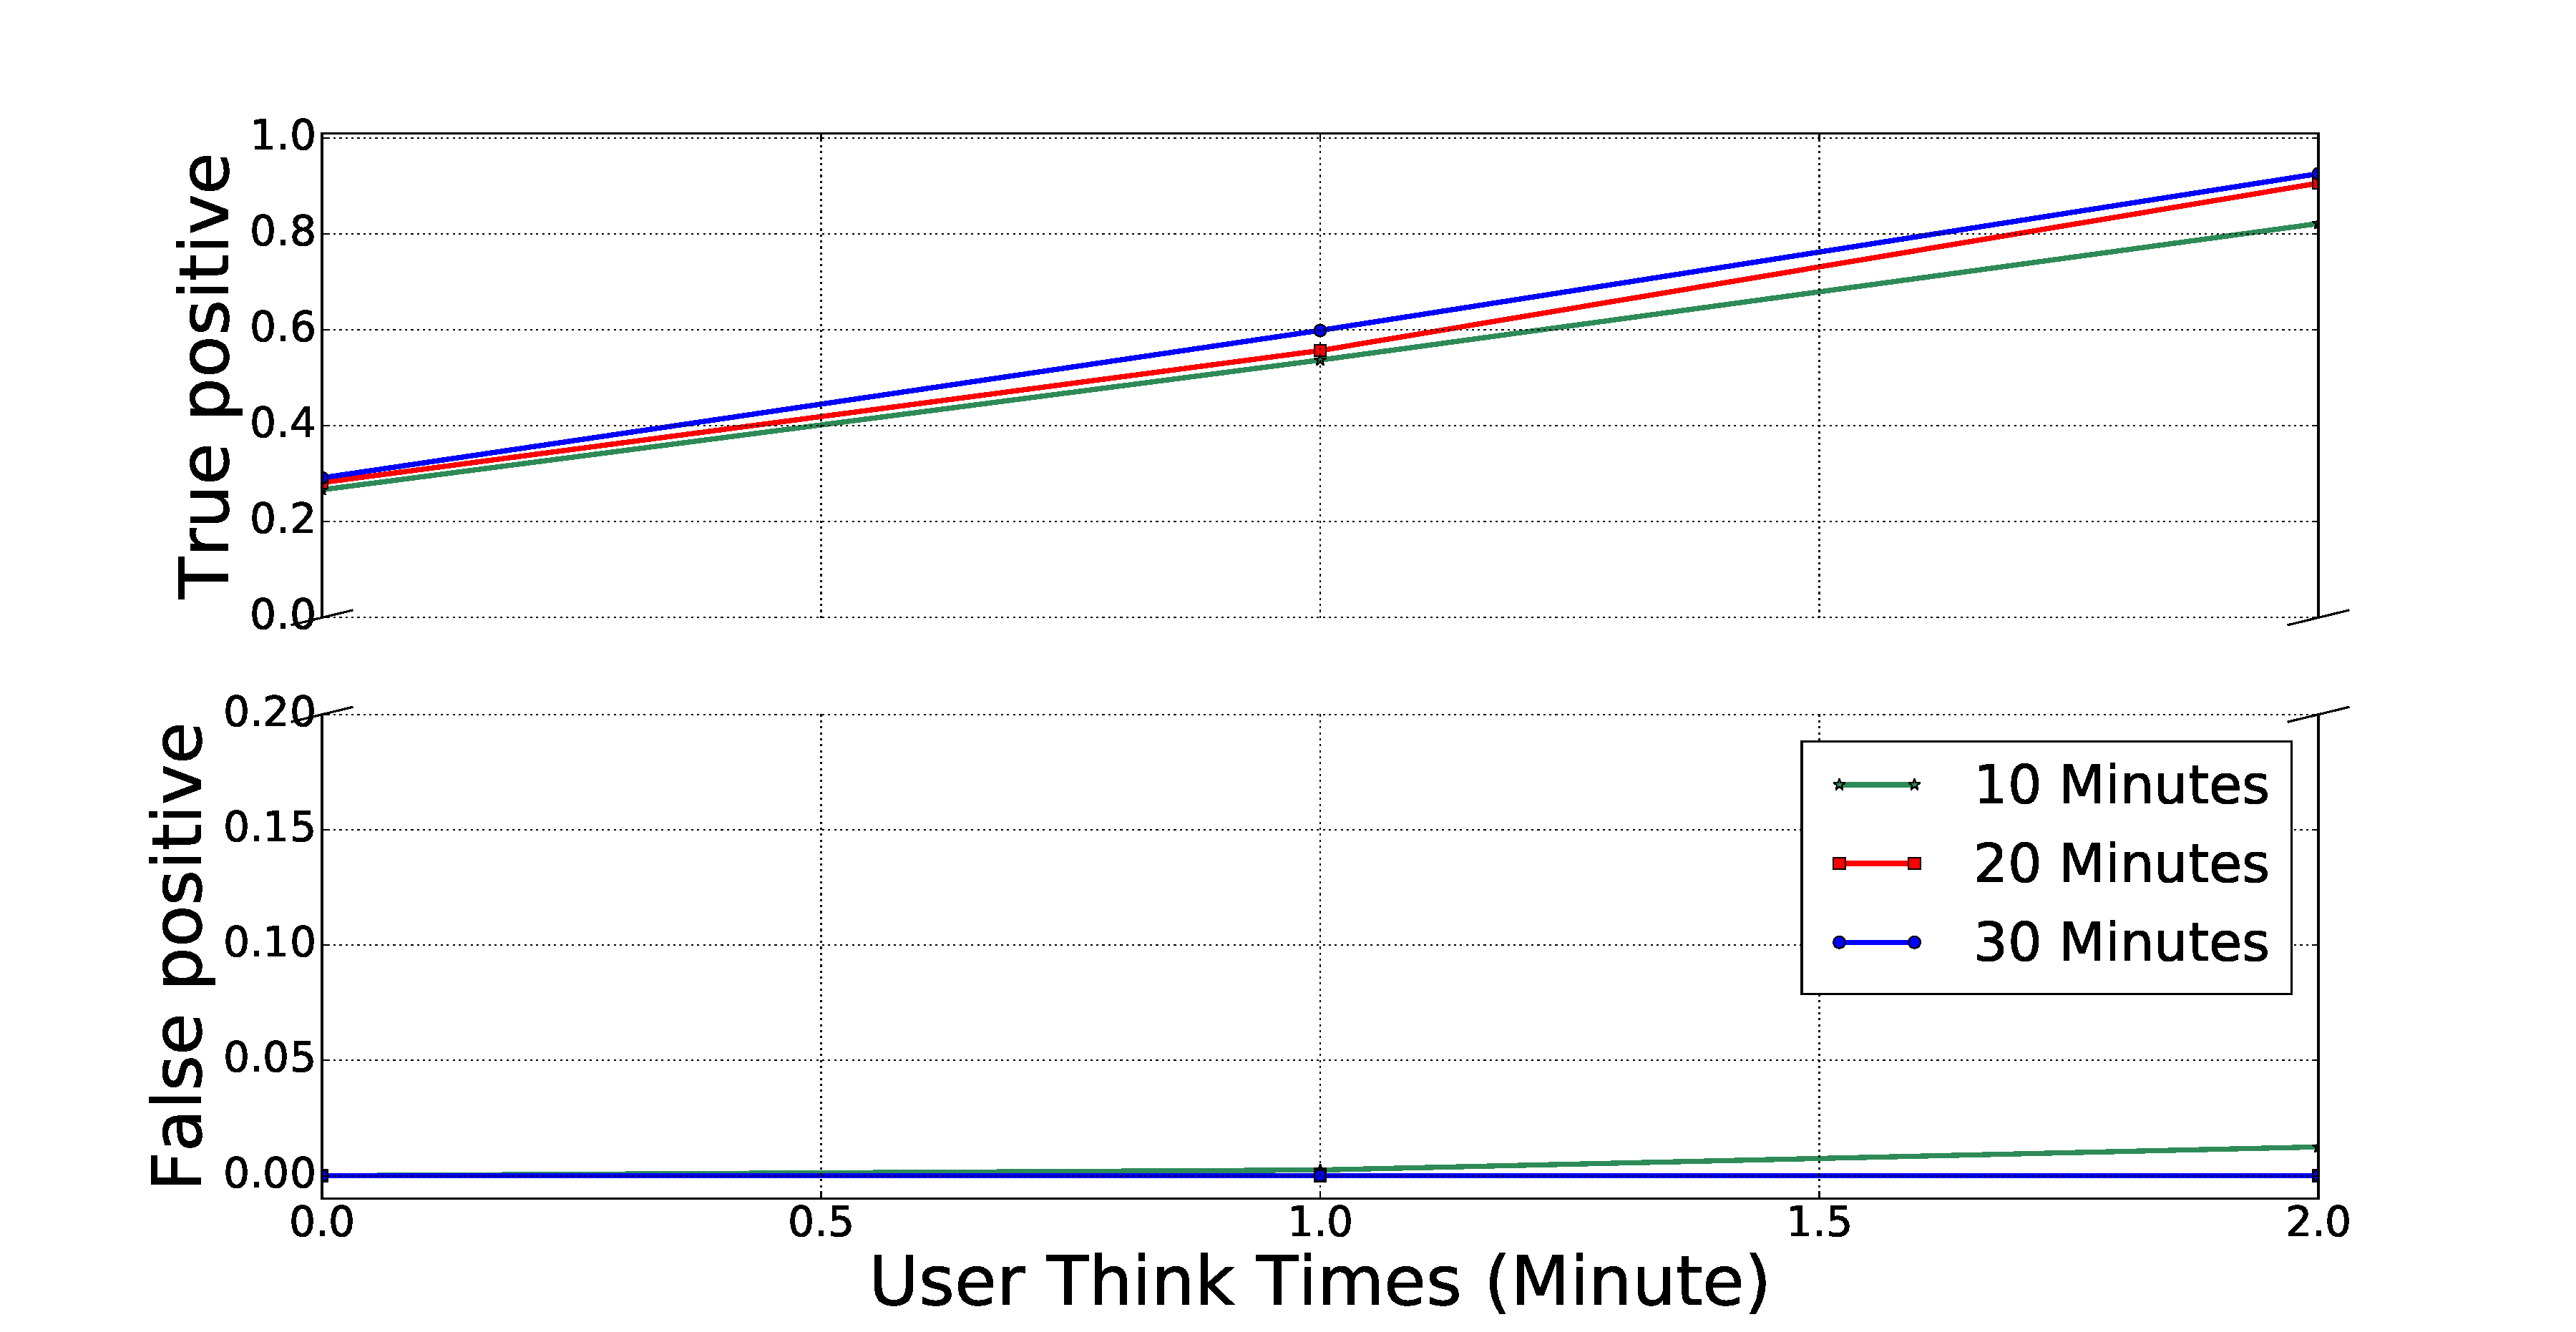
\includegraphics[width=\linewidth]{image/jan25/tor_all_sizehist.pdf}
\caption{SizeHist}
\label{fig:sizeHist}
\end{subfigure}
\caption{Detecting Bitcoin traffic behind Tor (Tor and its three pluggable transports: meek, obfs, fte) Using different classifiers}
\label{fig:vanilla_tor_effect_users}
\end{figure*} 
\end{comment}
\begin{comment}
In section~\ref{sec:exp}, we showed that our classifiers are able to detect \bc traffic with good accuracy.
As we noted before, some of our classifiers won't be able to detect \bc traffic when we add some cover traffic. But some of the classifiers resist in presence of large noise (neural net on Volume per sec). Here, we want to find possible countermeasures which would resist our classifiers.

Another possible countermeasure is to add some cover traffic to hide \bc traffic. We need to add as much traffic which is enough to dominates \bc traffic and thus, hide it. But at the same time, we do not want to add an enormous amount of traffic to have a high overhead. 
 The question that arises here is that: how much cover traffic do we need to hide \bc traffic. To find the minimum of cover traffic which hides \bc traffic, we do experiment with different amount of browsing traffic. 
\end{comment}
